%********************************************************************************
\documentclass[11pt,subeqn]{article}
\usepackage{etex}
\reserveinserts{28}

%-------------------------------------------------------------------------------
%--- PACKAGES
%-------------------------------------------------------------------------------
\usepackage{chronosys}
\usepackage{url}
\usepackage{longtable}
\usepackage{booktabs}
\usepackage{bold-extra}
\usepackage{rotating}
\usepackage{dcolumn}
%\usepackage{chronology}
\usepackage{color}
\pagecolor{white}
\usepackage{pdfpages}
\usepackage{lastpage}
\usepackage{lscape}
\usepackage{lineno}
\usepackage{setspace}
\usepackage{amsmath}
\usepackage{amssymb}
\usepackage{breqn}
\usepackage{appendix}
\usepackage{natbib}
\usepackage[capposition=top]{floatrow}
\usepackage{graphicx}
\usepackage{epsfig}
\usepackage{epstopdf}
\usepackage{multirow}
\usepackage{titletoc}
\usepackage{wrapfig}
\usepackage{blindtext}
\usepackage{subcaption}
\usepackage{subfloat}
\usepackage{xr}
\externaldocument{BentancorClarke_AdolescentFertility}

\definecolor{blue}{HTML}{84CECC}
\definecolor{gr}{HTML}{375D81}

%-------------------------------------------------------------------------------
%--- SPECIFICATIONS (MARGINS, TOC, BIBLIO)
%-------------------------------------------------------------------------------
\setlength\topmargin{-0.375in}
\setlength\textheight{8.8in}
\setlength\textwidth{5.8in}
\setlength\oddsidemargin{0.4in}
\setlength\evensidemargin{-0.5in}


\bibliographystyle{abbrvnat}
\bibpunct{(}{)}{;}{a}{,}{,}



\titlecontents{section}
[0pt]
{}%
{\contentsmargin{0pt}
    \thecontentslabel\enspace%
    }
{\contentsmargin{0pt}}
{\titlerule*[.5pc]{.}\contentspage}
[]

\renewcommand\figurename{Appendix Figure}
\renewcommand\tablename{Appendix Table}
\renewcommand\thesection{\Alph{section}}
\renewcommand*{\thepage}{A\arabic{page}}
\renewcommand*{\theequation}{A\arabic{equation}}


%-------------------------------------------------------------------------------
%--- FRONT PAGE
%-------------------------------------------------------------------------------
\begin{document}
\begin{spacing}{1.4}

\begin{center}
\textbf{ONLINE APPENDICES} \\
\vspace{4mm}
From the paper: \\
\vspace{6mm}
{\large \textsc{Assessing Plan B: 
The Effect of the Morning After Pill on Children and Women}} \\
Damian Clarke and Andrea Bentancor
\end{center}

\tableofcontents


%-------------------------------------------------------------------------------
%--- MAIN CONTENTS
%-------------------------------------------------------------------------------
\setlength\parindent{0.25in}
\setlength\parskip{0.25in}


\newpage
\section{Data Appendix}
\subsection{Births, Deaths and Population}
Population data from Chile comes from two main sources.  The first is vital 
statistics data, recording births and fetal deaths which are provided by the 
Ministry of Health of the Government of Chile (MINSAL).  This data provides 
microdata records covering greater than 99\% of all births and fetal deaths 
reported in aggregate data \citep{Bharadwajetal2013} in the country.  Each 
entry records the occurrence of a birth or fetal death, characteristics of the 
mother (and if present father) including her age, education, and muncipality of 
residence, as well as a number of charactersitics of the birth (including birth 
weight, gender, gestation and birth order) or the fetal death (weeks of 
gestation, birth order, ICD-10 code\footnote{The ICD (or Internation 
Classification of Disease) code is a standard set of codes which classify deaths 
according to their cause. These are used worldwide to facilitate classification 
and generation of national mortality statistics. The ICD-10 has been in use in
Chile to classify fetal (and all) deaths since 1997 \citep{INE2014}.}). These 
data have been collected and reported in Chile since 1982, and, at the time of 
writing, are publicly available online up to the year 2012 at the following url: 
\texttt{http:\/\/www.deis.cl\/?p=1020}.  These vital statistics data for birth 
and fetal deaths thus provide data on all pregnant women in the country who 
either give live birth, have a birth leading to fetal death or who miscarry in 
any hospital in the country. 

Data on all women of reproductive age comes from the National Institute of 
Statistics of Chile (INE). The INE provides estimations of the number of women 
of each age living in each municipality in each year.  These estimates are based 
on the decennial census, as well as net migration each year, and vital 
statistics on all births and deaths occurring to residents in the municipality 
\citep{INE2014}.  These two sources of data provide information on the number
of women of fertile age living in each municipality, and the number of women
pregnant in each municipality during the time period of interest.  They can be
merged at the level of the municipality, resulting in counts of total number of
births, fetal deaths, and women of each age, and hence a calculation of
municipal-level rates of pregnancy (births/total women), and fetal deaths
(fetal deaths/total births).

%Appendix tables \ref{strucTab} and \ref{reshapeTab} provide an excerpt of the
%structure of the data constructed using MINSAL vital statistics and INE 
%population records.  Municipal level data of population and total births are
%collected for each municipality, year and age group, and the number of 
%non-pregnant women is calculated by subtracting pregnant women from the total
%female population of this age (Appendix table \ref{strucTab}).  From this
%table rates and counts of births are known and OLS regressions can be run.  In 
%order to run a weighted binary regression, this table can be reshaped, to form
%records of the number of pregnant and non-pregnant women in each municipality,
%year and age group (Appendix table \ref{reshapeTab}).  In both cases, the data
%are matched at the level of the municipality, so all birth and population 
%records are successfully matched.
%
%\end{spacing}
%\begin{spacing}{1}
%\begin{table}[htpb!]
%\begin{center}
%\caption{Birth and Population Data (18 year olds)}
%\label{strucTab}
%\begin{tabular}{lccccc} \toprule
%Comuna & Year & Population & Pregnant & Not Pregnant & Rate \\ \midrule
%Arica & 2009 & 1575 & 119 & 1456 & 0.076 \\
%Arica & 2010 & 1579 & 118 & 1461 & 0.075 \\ 
%Arica & 2011 & 1534 & 116 & 1418 & 0.076 \\ \bottomrule
%\multicolumn{6}{p{11.2cm}}{\begin{footnotesize}\textsc{Note:} Column 3 is from INE, 
%column 4 from MINSAL. Non-pregnancies in Column 5 are calculated from birts and
%total women (Column 3$-$Column 4), and the rate is calcualted by taking the ratio
%of pregancies over total women (Column 4/Column 3).\end{footnotesize}}
%\end{tabular}
%\end{center}
%\end{table}
%
%\begin{table}[htpb!]
%\begin{center}
%\caption{Reshaped Data for Analysis (18 yo)}
%\label{reshapeTab}
%\begin{tabular}{lccc} \toprule
%Comuna & Year & Pregnant & Weight \\ \midrule
%Arica & 2009 & 1 & 119 \\
%Arica & 2009 & 0 & 1456 \\
%Arica & 2010 & 1 & 118 \\
%Arica & 2010 & 0 & 1461 \\
%Arica & 2011 & 1 & 116 \\
%Arica & 2011 & 0 & 1418 \\ \bottomrule
%\end{tabular} \\
%\end{center}
%\end{table}
%\end{spacing}
%\begin{spacing}{1.4}

%-------------------------------------------------------------------------------
We observe 1,605,300 live births and 13,063 fetal deaths occurring to 15-49 year 
old women from 2006-2012.  Appendix figure \ref{TEENfig:ageHist} plots the 
distribution of mother's age at birth in Chile over the period of study, while
appendix figure \ref{TEENfig:ageHistD} plots the distribution of fetal deaths by 
ages of the woman.  For births, the distribution is multi-modal, 
with a peak for women in their late teens and early 20s, and another peak in the 
late 20s.  As in the USA, the rate of fetal deaths are highest among teenage and 
older women \citep{MacDormanGregory2015}, with the absolute number in Chile 
being highest among young women.

\begin{figure}[htpb!]
\begin{center}
\caption{Frequency of Births by Mother's Age: Chile 2006-2012}
\label{TEENfig:ageHist}
\includegraphics[scale=0.44]{../Figures/ageDistBirths.pdf} 
\end{center}
\end{figure}

\begin{figure}[htpb!]
\begin{center}
\caption{Frequency of Fetal Deaths by Mother's Age: Chile 2006-2012}
\label{TEENfig:ageHistD}
\includegraphics[scale=0.44]{../Figures/ageDistDeaths.pdf} 
\end{center}
\vspace{-4mm}
\floatfoot{\textsc{Notes to Appendix figures \ref{TEENfig:ageHist}-
\ref{TEENfig:ageHistD}}: 
Sample consists of all births and fetal deaths (respectively) occurring in Chile
between the years of 2006-2012.  Data comes from the Ministry of Health of the
Government of Chile's vital statistics data.}
\end{figure}

The population of fertile-aged women in Chile during this period was 
approximately 4.25 million.\footnote{According to the 2002 census, the population
of Chile was 15,116,435, of which 50.7\% were women.  The most recent estimates
from INE are 17,556,815, and 50.5\% respectively.}  Over the entire period 
2006-2012, 29,801,999 fertile aged women were exposed (4.25 million women per 
year for 7 years).  Appendix figure \ref{TEENfig:Pregtime} displays pregnancy 
rates by age-group over the period of study, calculated from MINSAL vital
statistics and INE population data. These figures are virtually indistinguishable 
from rates published in aggregate data by MINSAL \citep{MINSAL2013} as well as
those published in The World Bank's Data Bank (indicator SP.ADO.TFRT).\footnote{%
For example, The Ministry of Health reports that the rate of pregnancy per 1,000
women aged 15-19 over the same period was: 51.0 per 1,000 in 2006, 53.4/1,000
in 2007, 54.9/1,000 in 2008, 54.3/1,000 in 2009, 52.0/1,000 in 2010, 
50.4/1,000 in 2011, and 48.6/1,000 in 2012.}  A similar figure for rates of
birth and death for the entire population under study is presented in the
body of the paper (figure \ref{TEENfig:BirthDeath}).

\begin{figure}[htpb!]
\begin{center}
\caption{Pregancies by Age Group and Time}
\vspace{-5mm}
\label{TEENfig:Pregtime}
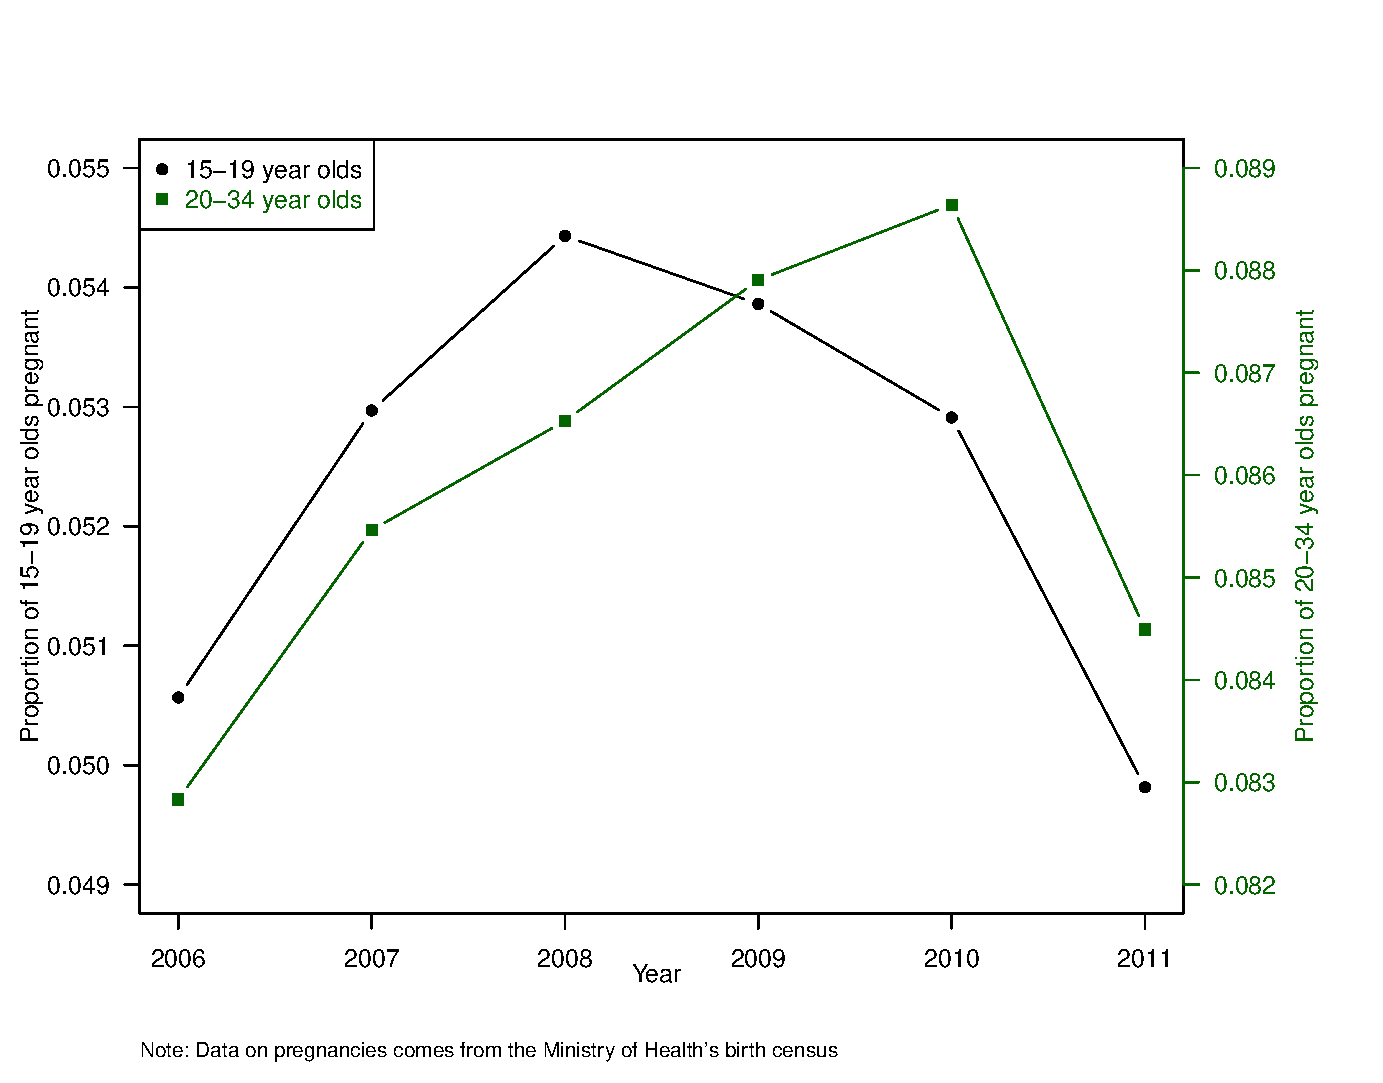
\includegraphics[scale=0.54]{../Figures/Births.eps} 
\end{center}
\end{figure}


\clearpage
\renewcommand\thesection{\Alph{section}}
\setlength\parindent{0.25in}
\setlength\parskip{0.25in}

\subsection{Distance to Treatment}
Distance-to-treatment analysis is run, to determine whether local spillovers
occur between EC pill and ``near to EC pill'' municipalities.  An expanded
explanation of equation \ref{TEENeqn:spillover} (from the paper) is provided
below.  This consists of defining a series of $close$ variables in the
following specification:
\begin{equation}
 \label{TEENeqn:spillover2}
y_{jt} = \alpha + \delta\cdot \mathbb{I}\{Pill_{jt-1}\} + 
	\sum_{c=0}^C\zeta_c\cdot close^c_{jt-1} + \phi_t + 
\eta_j + \eta_j\cdot t + X_{jt-1}\gamma + \varepsilon_{jt}.
\end{equation}
where
\[
 close^C_{jt} =
  \begin{cases}
   1 & \text{if } dist_{jt} > c \wedge dist_{jt}\leq c+k   \\
   0 & \text{if } dist_{jt} \leq c \vee  dist_{jt}>c+k.
  \end{cases}
\]
where $dist_{jt}$ is the distance (in km) to the nearest treatment municipality 
(ie a municipality which reports prescribing the pill)\footnote{In theory, we
will also be concerned if the distance to a national border is small, and women
can easily cross the national border to gain access to the EC pill.  In practice
in Chile this is not a major concern given that arriving to Argentina (which
\emph{does} provide access to the EC pill requires crossing the Andes, and 
Chile's two other neighbours: Bolivia and Peru, either do not prescribe the EC
pill (Bolivia), or require a national identity card for access (Peru).} and 
$k$ is a bandwidth-type parameter.  We define $k$ as 10, so close is defined
as a dummy for living withing (0,10]km, (10,20]km, and (20,30]km from the
nearest EC pill municipality.

Spillover analysis in section \ref{TEENsscn:spillover} of the paper requires
data on the distance of each non-treatment municipality to the nearest 
treatment municipality.  Principal measures of distance from treatment is 
calculated by using GIS software to take a Euclidean distance from the 
centroid of non-treatment municipalities, to the centroid of the nearest 
municipality which did offer the morning after pill in each year under 
study.\footnote{In order to calculate distances, the official map shape file
from the Chilean Library of Congress was consulted, which available on the
web at \texttt{http://siit2.bcn.cl/mapas_vectoriales}.}  The distribution of
distances from each non-treatment municipality to its nearest treatment 
municipality in kilometres is presented in Appendix figure \ref{dist}.

As a robustness check, alternative distance measures were also used.
Firstly, we collated the shortest distance over roads from non-teatment to 
treatment municipalities.  This was calculated using repeated calls to the 
Google Distance Matrix API,\footnote{Full details can be found at:
\url{https://developers.google.com/maps/documentation/distancematrix/\#api\_key}.
I have made the computational routine used available on the web at:
\url{https://github.com/damiancclarke/spillovers/blob/master/source/distCalc/queryDist.py}.}
which finds the shortest path over roads.  In the case of Chile, this requires 
calculating the distances between all 346 municipalities ($346^2/2=$59,858
distance pairs) in each year.  Secondly, rather than distance in 
kilometres, as in Euclidean or road distance, a measure of travel \emph{time} 
was calculated.  As a proxy for total travel time, travel time by car was 
caclulated between areas.  This was similarly generated using calls to Google 
Maps, resulting in one value for each municipality pair (see example in Appendix
Figure \ref{googdist}).  In each case ``distance to treatment'' is then the 
minimum value to the nearest treatment area, which varies by municipality and 
year.  Appendix Figure \ref{altdist} displays the distribution of alternative
distance measures for shortest distance over roads, and travel time in car.

\begin{figure}[htpb!]
\includegraphics[scale=0.55]{../Figures/EuclideanDistance.eps}
\caption{Simple Distance to Treatment}
\label{dist}
\floatfoot{\textsc{Notes to figures \ref{dist}}: 
Histogram presents the distance from each municipality where the pill
was not available to the closest pill municipality in the years 2009-2011.
Distances over 150 km have been omitted for clarity.  Less than 1.5\% of 
non-pill municipalities are greater than 150km from the nearest pill 
municipality.}
\end{figure}

\begin{figure}[htpb!]
\includegraphics[scale=0.7]{../Figures/mapDistance.png}
\caption{Distance based on googlemaps}
\label{googdist}
\end{figure}

\begin{figure}[htpb!]
\begin{center}
\caption{Alternative Measures of Distance to Treatment}
\label{altdist}
\begin{subfigure}{.5\textwidth}
  \centering
  \includegraphics[scale=0.32]{../Figures/TravelTime.eps}
  \caption{Travel time by vehicle}
  \label{travelTime}
\end{subfigure}%
\begin{subfigure}{.5\textwidth}
  \centering
  \includegraphics[scale=0.32]{../Figures/RoadDistance.eps}
  \caption{Distance over roads}
  \label{roadDist}
\end{subfigure}
\end{center}
\vspace{-4mm}
\floatfoot{\textsc{Notes to figures \ref{altdist}}: 
Histograms present the distance from each municipality where the pill
was not available to the closest pill municipality in the years 2009-2011.
Distances over 150 km (minutes) have been omitted for clarity.  In each 
case, less than 1.5\% of non-pill municipalities are greater than 150km 
(minutes) from the nearest pill municipality.}
\end{figure}

These alternative measures of distance do not majorly affect the quantitative 
implication of findings reported in the paper.  Appendix tables 
\ref{TEENtab:SpilloverRoad} and \ref{TEENtab:SpilloverTime} replicate table 
\ref{TEENtab:Spillover} from the paper, replacing Euclidean distance with 
distance over roads, or travel time in car. Results from both tables suggest 
a treatment effect of approximately 3.5 fewer births per 1,000 women aged
15-19 once accounting for spillovers of 30 minutes travel time or
30km of distance respectively, following the spillover methodology outlined
in the paper.

\clearpage
\subsection{Time-Varying Municipality and Region Controls}
Time-varying municipal controls such as education and health spending, and the
number of females working in public government is downloaded from the National
System of Municipal Information (SINIM).  This provides data as far back as
2005, and is freely available for download online at
\url{http://www.sinim.gov.cl/indicadores/busq_serie.php}.

Data on municipal elections, mayor's gender, party and vote share is accessed
from the Electoral Service of Chile (SERVEL).  This provides all electoral
results from municipal elections for the full time period of this study.  Raw
data is available online at 
\url{http://www.servel.cl/ss/site/mobile/padron_electoral_comunal_por_ano_informe_comunal_anual.html}
or processed as one line per municipality at the data page of the author
(Clarke's) webiste: \url{github.com/damiancclarke/morning-after-pill}.

Finally, we calculate data for alternative contraceptive use based on
a series of regionally representative surveys collected every 3 years beginning
in 1994.  The National Survey of Youth asks respondents whether they use any 
method of contraception in both their first and most recent sexual activity.  
In the case that they did not use a condom, they are asked whether this is 
because they did not have access.  Based on this survey, access to condom is
calculated as an additional time-varying control.  However, it should be noted
that this variable can only be calculated at the level of the region (one
geographic level above the municipality), given that this survey is not
representative at the level of the municipality.  Once again, processed data and
processing scripts are made available at the data section of the author's site,
and, if desired, raw data is available on the web: 
\url{http://extranet.injuv.gob.cl/Encuesta_Nacional_de_la_Juventud/contenido/index.php}.

\clearpage
\section[Additional Details of the Emergency Contraceptive Reform]{The Chilean 
Legislative Environment and the Adoption of Emergency Contraception}
\label{TEENscn:applegislate}
Discussions surrounding the introduction of emergency contraception in Chile
have taken place since at least 1996, when the Chilean Institute of 
Reproductive Medicine (ICMER for its initials in Spanish) proposed the use of
this method to avoid undesired pregnancies in a country where abortion was
entirely outlawed \citep{Dides2009}.  However, the first legislative attention
given to this matter occurred when the aforementioned (see section 
\ref{TEENsscn:Chile}) Institute of Public Health emitted a resolution allowing
for the production and sale of `Postinol', a drug containing levonogestrel by a
Chilean laboratory in 2001.  The Constitionality of this was quickly 
challenged, and the drug was prohibited by the Supreme Court.

The emergency contraceptive pill again entered legislative attention in 2004,
following the Ministry of Health's publication of a guide suggesting that 
emergency contraception be used following cases of rape.  Following this in 
2005, the Subsecretary of Health Dr.\ Antonio Infante announced that emergency
contraception would be freely available to \emph{all} women who requested it,
however the President of Chile and the Ministry of Health later declared that
this was not the case, leading to removal of the Subsecretary from office.

In November of 2005, the Supreme Court of Chile provided the first 
constitutional support for the emergency contraceptive pill, voting 5-0 to
reverse the decision taken in 2001, allowing emergency contraception to be
provided in the case that the mother's life was in danger.  Once again however,
this finding was challenged shortly thereafter.  The same non-governmental 
institution which had earlier raised a case against ICMER, now challenged the 
private commercial laboratory in charge of producing and distributing the drug.  
However, before this case could reach court, this laboratory voluntarily gave 
up their license to produce the drug, in a three line statement issued by the
General Director of the company on February 14, 2006 \citep{CasasBecerra2008}.

In the same year, a group of 36 parliamentary deputies from conservative 
parties raised a case with the Constitional Tribunal, claiming that the 
provision of the emergency contraceptive pill contravened the ``National Laws
for the Regulation of Fertility'', a set of rules issued by the Ministry of
Health.  This case was only resolved in 2008, with the Constitional Tribunal's
finding in favour of this group, hence making illegal any provision by 
hospitals or health centres controlled by the Ministry of Health (and hence
under the jurisdiction of the National Fertility Laws).  Fundamentally however,
this left the door open for Municipal health centres to distribute the pill
freely to women.  These Municipal Health Centres are run under the directive
of the elected mayor of each Municipality, leaving all remaining legislation 
regarding the distribution of the pill up to the 346 mayors in Chile.

In this study we focus on the period surrounding this 2008 legislation as the 
cutoff of interest.  However, even after this finding the emergency 
contraceptive pill has not been far from legislative action, with a number of
other cases raised.  These cases never entirely threatened the continuity of
supply of the morning after pill by municipalities, however did cause some
confusion for mayors and municipal health bodies in determining whether or not
they were legally allowed to prescribe the contraceptive.  These cases also
resulted in the passing of a number of laws and standards.  Most importantly,
they resulted in national Law 20.418 which ``creates standards for information,
guidance and regulatory services in fertility'' (author's translation), and 
the passing of a decree on March 3, 2013, which makes obligatory the provision
of the morning after pill to women of any age in any health centre in Chile.  
This became operative on May 28, 2013, meaning that---at least officially---%
there are no longer any restrictions in place in the country.

While the morning after pill was only legalised in Chile with these reforms,
the functionality of the morning after pill (the prevention of ovulation) can
be simulated using an overdose of the traditional oral contraceptive pill 
\citep{TaskForce1998}\footnote{This method is not as effective as more 
modern regimes which are based on levonorgestrel (LNG). The 
\citeauthor{TaskForce1998}'s estimates suggest that the use of LNG results in
87\% effectiveness, while the Yuzpe method is 57\% effective. The Yuzpe regime
is also trickier to follow as it requires two doses seperated by 12 hours, and
is associated with higher rates of naseau.}. This is known as the Yuzpe method, 
or the Yuzpe regime. We are not aware of any evidence or survey data which exists 
to determine the knowledge of this method among the population of Chilean women.  
However, if the arrival of the morning after pill reform also brings with it 
greater awareness of the Yuzpe method, we may be concerned that we mistakenly 
infer that this is the effect of the EC pill itself, and not increased knowledge 
of alternative methods.  However, in searching through many official government 
documents and unofficial documents both prior and posterior to the reform, we 
find little evidence to suggest that this was a widely discussed or suggested 
method.  In both the 2006 and 2012 revisions of the National Laws for the 
Regulation of Fertility, as well as the Ministry of Health's Manual on Teenage 
Pregnancy, no mention of this method was made (however the EC pill was mentioned 
in the 2012 revision of the law as well as the Manual on Teenage Pregnancy). In 
the only survey data of which we are aware which asks about the Yuzpe method 
\citep{Didesetal2010}, of 162 surveyed municipal health centres, only 3 of 
these mention suggesting the Yuzpe method if the EC pill is not available.  Our 
reading of the source documents and data suggests that there is no reason to 
think that the reform is associated with a change in the frequency of the Yuzpe 
method, or that the Yuzpe method was widely discussed in Chile.

\begin{figure}
\startchronology[align=left, startyear=2004,stopyear=2015, height=0pt, startdate=false, stopdate=false, dateselevation=1pt, arrow=false, box=true]
%\chronograduation[event][dateselevation=0pt]{2}
\chronoperiode[textstyle=\raggedleft\colorbox{gr!50}, color=gr, startdate=false, bottomdepth=0pt, topheight=8pt, textdepth=-25pt,dateselevation=16pt, stopdate=false]{2008}{2012}{Municipal variation in provision}
\chronoperiode[textstyle=\colorbox{blue!50}, color=blue, startdate=false, bottomdepth=8pt, topheight=16pt, textdepth=-18pt, dateselevation=12pt, stopdate=false]{2004}{2008}{No EC in Health Centres}
\chronoevent{2013}{Nationally Available}
\chronoevent{2008}{\textbf{Reform}: Constitutional Finding}
%\chronoevent{2012}
\stopchronology
%%%
%%%\begin{chronology}[2]{2004}{2015}{10cm}
%%%\event{2008}{\textbf{Reform}: Constitutional Finding}
%%%\event[2008]{2012}{Municipal-variation in EC provision}
%%%\event{\decimaldate{3}{3}{2013}}{Nationally Available}
%%%\end{chronology}
\caption{Timing of the Reform}
\label{TEENfig:reformtiming}
\floatfoot{\textsc{Notes to figure \ref{TEENfig:reformtiming}:} Prior to 2008, the
EC pill was not available at any health care centres or hospitals, and was only
very infrequently available for purchase at pharmacies.  Between 2008 and 2012, the
EC pill was freely available in municipal health centres only if the mayor of the
municipality directed centres to provide it.  Over this period, a given municipality
could change their decision, and if prescribing in one year, did not necessarily
prescribe the next year.  From 2013 onwards, the EC pill was legally available for
free in all municipalities, and from 2015 onwards, was available for purchase in all
pharmacies without a prescription.}
\end{figure}


\clearpage
\section{Alternative Specifications and Tests}
\textbf{Notes for appendix tables}\\
Appendix Table \ref{TEENtab:aggregateASFRunweight}: Full OLS
regressions of age-specific fertility rate (ASFR) and gross fertility
rate (GFR) at the municipality level, not weighted for municipal
population. Partial results are displayed in the main paper, in table 
\ref{TEENtab:BirthRobust}.

\noindent Appendix table \ref{TEENtab:aggregateLog}: Full OLS regressions 
of the log(number of births + 1) at the level of the municipality, with
FEs, trends and time varying controls.  Referred to in section 
\ref{TEENsscn:rbirths} of the main paper, and partial results are
displayed in the main paper, in table 
\ref{TEENtab:BirthRobust}.

\noindent Appendix table \ref{TEENtab:aggregateLogunweight}: Identical
to appendix table \ref{TEENtab:aggregateLog}, however with no weighting
for municipal population.

\noindent Appendix table \ref{TEENtab:aggregate}: Identical to appendix
table \ref{TEENtab:aggregateLog}, but using the number rather than the log
number of births.  Partial results are displayed in the main paper, in 
table \ref{TEENtab:BirthRobust}.

\noindent Appendix table \ref{TEENtab:aggregateunweight}: Identical
to appendix table \ref{TEENtab:aggregate}, however with no weighting
for municipal population.

\noindent Appendix Table \ref{TEENtab:DeathOLSunweight}: Full OLS
regressions of deaths per live birth at the municipality level with FEs,
trends, and time varying controls, but not weighted by municipality
population. Weighted table is presented as table \ref{TEENtab:DeathOLS}
in the main paper.

%%\noindent Appendix table \ref{TEENtabPregFull}: Identical to main weighted
%%logit presented in the paper for the effect of the EC pill on births with 
%%full controls, however displaying all control variables in output.
%%
%%\noindent Appendix table \ref{TEENtabDeathFull}: Identical to main weighted
%%logit presented in the paper for the effect of the EC pill on early term
%%fetal deaths with full controls, however displaying all control variables in 
%%output.

\noindent Appendix table \ref{TEENtab:SpilloverRoad}: Identical to main 
spillover table in body of the paper (table \ref{TEENtab:Spillover}), but 
rather than measuring distance to treatment as the Euclidean distance from 
the centroid of each municipality, distance is measured as kilometres 
travelled over roads.

\noindent Appendix table \ref{TEENtab:SpilloverTime}: Identical to main 
spillover table in body of the paper (table \ref{TEENtab:Spillover}), but 
rather than measuring distance to treatment as the Euclidean distance from 
the centroid of each municipality, distance is measured as total travel time
expected in vehicle.


\begin{table}[!htbp] \centering
\caption{The Effect of the EC Pill on Birth Rates (Unweighted)}
\label{TEENtab:aggregateASFRunweight}
\begin{tabular}{@{\extracolsep{5pt}}lcccc}
\\[-1.8ex]\hline \hline \\[-1.8ex] 
& Birth& Birth& Birth& Birth\\
& Rate & Rate & Rate & Rate \\
&(1)&(2)&(3)&(4) \\ \hline
\multicolumn{5}{l}{\noindent \textbf{
Panel A: All Women}} \\
Emergency Contraceptive Pill&$-$0.282&$-$1.600$^{***}$&$-$1.284$^{***}$&$-$1.789$^{***}$\\
            &[0.641]&[0.290]&[0.314]&[0.437]\\
 & & & & \\
Observations&2,210&2,210&2,210&2,210\\
Mean Birth Rate&53.87&53.87&53.87&53.87\\
 & & & & \\
\multicolumn{5}{l}{\noindent \textbf{
Panel B: 15-19 year olds}} \\
Emergency Contraceptive Pill&$-$2.778$^{***}$&$-$2.871$^{***}$&$-$2.219$^{***}$&$-$3.527$^{***}$\\
            &[0.489]&[0.501]&[0.561]&[0.700]\\
 & & & & \\
Observations&2,205&2,205&2,205&2,205\\
Mean Birth Rate   &52.00&52.00&52.00&52.00\\
 & & & & \\
\multicolumn{5}{l}{\noindent \textbf{
Panel C: 20-34 year olds}} \\
Emergency Contraceptive Pill&$-$1.288&$-$2.751$^{***}$&$-$2.255$^{***}$&$-$3.106$^{***}$\\
            &[1.134]&[0.515]&[0.580]&[0.810]\\
 & & & & \\
Observations&2,210&2,210&2,210&2,210\\
Mean Birth Rate   &85.49&85.49&85.49&85.49\\
 & & & & \\
\multicolumn{5}{l}{\noindent \textbf{
Panel B: 35-49 year olds}} \\
Emergency Contraceptive Pill&0.670$^{*}$&$-$0.204&$-$0.129&0.099\\
            &[0.379]&[0.211]&[0.218]&[0.267]\\
 & & & & \\
Observations&2,210&2,210&2,210&2,210\\
Mean Birth Rate&21.40&21.40&21.40&21.40\\
\hline \\[-1.8ex] 
{\small Year \& Comuna FEs}             &Y&Y&Y&Y \\
{\small Municipal-Specific Linear Trends}& &Y&Y&Y \\
{\small Time Varying Controls}           & & &Y&Y \\
{\small Spillovers}                      & & & &Y \\
\hline \hline \\[-1.8ex]
\multicolumn{5}{p{13.8cm}}{\begin{footnotesize}
\textsc{Notes:} Each panel presents unweighted       
difference-in-difference results for a regression of  
age-specific fertility rates (ASFR) on the EC reform  
for the age group 
in each municipality.  Specifications are identical to
 table \ref{TEENtab:aggregateASFR}, however are not  
weighted for population. Standard errors are clustered
at the level of the municipality.
$^{*}$p$<$0.1; $^{**}$p$<$0.05; $^{***}$p$<$0.01\end{footnotesize}}
\normalsize\end{tabular}\end{table}

\begin{table}[!htbp] \centering
\caption{The Effect of the EC Pill on log Births}
\label{TEENtab:aggregateLog}
\begin{tabular}{@{\extracolsep{5pt}}lcccc}
\\[-1.8ex]\hline \hline \\[-1.8ex] 
& ln(Birth) & ln(Birth) & ln(Birth) & ln(Birth) \\
&(1)&(2)&(3)&(4) \\ \hline
\multicolumn{5}{l}{\textbf{
\noindent Panel A: All Women}} \\
Emergency Contraceptive Pill&$-$0.026$^{***}$&$-$0.046$^{***}$&$-$0.029$^{***}$&$-$0.029$^{**}$\\
            &[0.008]&[0.010]&[0.010]&[0.012]\\
 & & & & \\
Observations&2,210&2,210&2,210&2,210\\
Mean of ln(Births+1) &7.37&7.37&7.37&7.37\\
 & & & & \\
\multicolumn{5}{l}{\noindent \textbf{
Panel B: 15-19 year olds}} \\
Emergency Contraceptive Pill&$-$0.113$^{***}$&$-$0.089$^{***}$&$-$0.055$^{***}$&$-$0.064$^{***}$\\
            &[0.012]&[0.020]&[0.020]&[0.024]\\
 & & & & \\
Observations&2,205&2,205&2,205&2,205\\
Mean of ln(Births+1) &5.46&5.46&5.46&5.46\\
 & & & & \\
\multicolumn{5}{l}{\noindent \textbf{
Panel C: 20-34 year olds}} \\
Emergency Contraceptive Pill&$-$0.009&$-$0.036$^{***}$&$-$0.024$^{**}$&$-$0.025$^{*}$\\
            &[0.009]&[0.011]&[0.012]&[0.014]\\
 & & & & \\
Observations&2,210&2,210&2,210&2,210\\
Mean of ln(Births+1) &7.02&7.02&7.02&7.02\\
 & & & & \\
\multicolumn{5}{l}{\noindent \textbf{
Panel B: 35-49 year olds}} \\
Emergency Contraceptive Pill&0.000&$-$0.032&$-$0.022&$-$0.010\\
            &[0.012]&[0.020]&[0.021]&[0.026]\\
 & & & & \\
Observations&2,210&2,210&2,210&2,210\\
Mean of ln(Births+1) &5.55&5.55&5.55&5.55\\
\hline \\[-1.8ex] 
{\small Year \& Comuna FEs}             &Y&Y&Y&Y \\
{\small Municipal-Specific Linear Trends}& &Y&Y&Y \\
{\small Time Varying Controls}           & & &Y&Y \\
{\small Spillovers}                      & & & &Y \\
\hline \hline \\[-1.8ex]
\multicolumn{5}{p{13.8cm}}{\begin{footnotesize}
\textsc{Notes:} Each panel presents population       
weighted difference-in-difference results for a       
regression of the log(Births+1) for the age group in  
each  municipality. Specifications are identical to   
table \ref{TEENtab:aggregateASFR}, however logs are  
 used in place of birth rates. Standard errors are    
clustered at the level of the municipality.
$^{*}$p$<$0.1; $^{**}$p$<$0.05; $^{***}$p$<$0.01\end{footnotesize}}
\normalsize\end{tabular}\end{table}

\begin{table}[!htbp] \centering
\caption{The Effect of the EC Pill on log Births (Unweighted)}
\label{TEENtab:aggregateLogunweight}
\begin{tabular}{@{\extracolsep{5pt}}lcccc}
\\[-1.8ex]\hline \hline \\[-1.8ex] 
& ln(Birth)&ln(Birth)&ln(Birth)&ln(Births) \\
&(1)&(2)&(3)&(4) \\ \hline
\multicolumn{5}{l}{\textbf{
\noindent Panel A: All Women}} \\
Emergency Contraceptive Pill&0.007&$-$0.037$^{***}$&$-$0.030$^{***}$&$-$0.039$^{***}$\\
            &[0.007]&[0.006]&[0.007]&[0.009]\\
 & & & & \\
Observations&2,210&2,210&2,210&2,210\\
Mean of ln(Births+1)&7.37&7.37&7.37&7.37\\
 & & & & \\
\multicolumn{5}{l}{\noindent \textbf{
Panel B: 15-19 year olds}} \\
Emergency Contraceptive Pill&$-$0.081$^{***}$&$-$0.076$^{***}$&$-$0.058$^{***}$&$-$0.079$^{***}$\\
            &[0.008]&[0.011]&[0.012]&[0.016]\\
 & & & & \\
Observations&2,205&2,205&2,205&2,205\\
Mean of ln(Births+1)&5.46&5.46&5.46&5.46\\
 & & & & \\
\multicolumn{5}{l}{\noindent \textbf{
Panel C: 20-34 year olds}} \\
Emergency Contraceptive Pill&0.020$^{***}$&$-$0.033$^{***}$&$-$0.028$^{***}$&$-$0.038$^{***}$\\
            &[0.007]&[0.006]&[0.007]&[0.011]\\
 & & & & \\
Observations&2,210&2,210&2,210&2,210\\
Mean of ln(Births+1)&7.02&7.02&7.02&7.02\\
 & & & & \\
\multicolumn{5}{l}{\noindent \textbf{
Panel B: 35-49 year olds}} \\
Emergency Contraceptive Pill&0.025$^{**}$&$-$0.021$^{**}$&$-$0.016&$-$0.004\\
            &[0.011]&[0.011]&[0.010]&[0.013]\\
 & & & & \\
Observations&2,210&2,210&2,210&2,210\\
Mean of ln(Births+1)&5.55&5.55&5.55&5.55\\
\hline \\[-1.8ex] 
{\small Year \& Comuna FEs}             &Y&Y&Y&Y \\
{\small Municipal-Specific Linear Trends}& &Y&Y&Y \\
{\small Time Varying Controls}           & & &Y&Y \\
{\small Spillovers}                      & & & &Y \\
\hline \hline \\[-1.8ex]
\multicolumn{5}{p{13.6cm}}{\begin{footnotesize}
\textsc{Notes:} Each panel presents unweighted       
difference-in-difference results for a regression of  
the total log(Births+1) for the age group in each     
 municipality. Specifications are identical to table  
\ref{TEENtab:aggregateLog}, however unweighted       
municipality averages are used. Standard errors are   
clustered at the level of the municipality.
$^{*}$p$<$0.1; $^{**}$p$<$0.05; $^{***}$p$<$0.01\end{footnotesize}}
\normalsize\end{tabular}\end{table}

\begin{table}[!htbp] \centering
\caption{The Effect of the EC Pill on Total Births}
\label{TEENtab:aggregate}
\begin{tabular}{@{\extracolsep{5pt}}lcccc}
\\[-1.8ex]\hline \hline \\[-1.8ex] 
& Number& Number & Number & Number \\
& Births& Births & Births & Births \\
&(1)&(2)&(3)&(4) \\ \hline
\multicolumn{5}{l}{\textbf{
\noindent Panel A: All Women}} \\
Emergency Contraceptive Pill&7.623&$-$27.564$^{***}$&$-$20.337$^{***}$&$-$25.936$^{***}$\\
            &[5.720]&[5.242]&[5.954]&[8.511]\\
 & & & & \\
Observations&2,210&2,210&2,210&2,210\\
Mean Number of Births&2632.67&2632.67&2632.67&2632.67\\
 & & & & \\
\multicolumn{5}{l}{\noindent \textbf{
Panel B: 15-19 year olds}} \\
Emergency Contraceptive Pill&$-$8.618$^{***}$&$-$8.519$^{***}$&$-$5.583$^{***}$&$-$7.474$^{***}$\\
            &[1.233]&[1.517]&[1.716]&[2.275]\\
 & & & & \\
Observations&2,205&2,205&2,205&2,205\\
Mean Number of Births&386.14&386.14&386.14&386.14\\
 & & & & \\
\multicolumn{5}{l}{\noindent \textbf{
Panel C: 20-34 year olds}} \\
Emergency Contraceptive Pill&11.605$^{***}$&$-$16.644$^{***}$&$-$12.890$^{***}$&$-$17.893$^{***}$\\
            &[4.173]&[3.621]&[4.257]&[6.101]\\
 & & & & \\
Observations&2,210&2,210&2,210&2,210\\
Mean Number of Births&1833.11&1833.11&1833.11&1833.11\\
 & & & & \\
\multicolumn{5}{l}{\noindent \textbf{
Panel B: 35-49 year olds}} \\
Emergency Contraceptive Pill&4.636$^{***}$&$-$2.401$^{*}$&$-$1.843&$-$0.541\\
            &[1.608]&[1.299]&[1.371]&[1.742]\\
 & & & & \\
Observations&2,210&2,210&2,210&2,210\\
Mean Number of Births&435.78&435.78&435.78&435.78\\
\hline \\[-1.8ex] 
{\small Year \& Comuna FEs}             &Y&Y&Y&Y \\
{\small Municipal-Specific Linear Trends}& &Y&Y&Y \\
{\small Time Varying Controls}           & & &Y&Y \\
{\small Spillovers}                      & & & &Y \\
\hline \hline \\[-1.8ex]
\multicolumn{5}{p{14.2cm}}{\begin{footnotesize}
\textsc{Notes:} Each panel presents population       
weighted difference-in-difference results for a       
regression of the total number of births for the age  
group in each municipality. Specifications are        
identical to table \ref{TEENtab:aggregateASFR},      
however birth weights are replaced by the total number
 of births. Standard errors are clustered             
at the level of the municipality.
$^{*}$p$<$0.1; $^{**}$p$<$0.05; $^{***}$p$<$0.01\end{footnotesize}}
\normalsize\end{tabular}\end{table}

\begin{table}[!htbp] \centering
\caption{The Effect of the EC Pill on Total Births (Unweighted)}
\label{TEENtab:aggregateunweight}
\begin{tabular}{@{\extracolsep{5pt}}lcccc}
\\[-1.8ex]\hline \hline \\[-1.8ex] 
& Number& Number & Number & Number \\
& Births& Births & Births & Births \\
&(1)&(2)&(3)&(4) \\ \hline
\multicolumn{5}{l}{\textbf{
\noindent Panel A: All Women}} \\
Emergency Contraceptive Pill&22.657&$-$106.553$^{***}$&$-$84.159$^{***}$&$-$127.625$^{***}$\\
            &[18.425]&[33.291]&[28.742]&[47.587]\\
 & & & & \\
Observations&2,210&2,210&2,210&2,210\\
Mean Number of Births&2632.67&2632.67&2632.67&2632.67\\
 & & & & \\
\multicolumn{5}{l}{\noindent \textbf{
Panel B: 15-19 year olds}} \\
Emergency Contraceptive Pill&$-$26.677$^{***}$&$-$30.429$^{***}$&$-$21.123$^{***}$&$-$31.887$^{***}$\\
            &[6.063]&[9.170]&[6.704]&[9.894]\\
 & & & & \\
Observations&2,205&2,205&2,205&2,205\\
Mean Number of Births&386.14&386.14&386.14&386.14\\
 & & & & \\
\multicolumn{5}{l}{\noindent \textbf{
Panel C: 20-34 year olds}} \\
Emergency Contraceptive Pill&42.779$^{***}$&$-$68.108$^{***}$&$-$58.777$^{***}$&$-$94.493$^{**}$\\
            &[15.774]&[20.798]&[21.672]&[37.084]\\
 & & & & \\
Observations&2,210&2,210&2,210&2,210\\
Mean Number of Births&1833.11&1833.11&1833.11&1833.11\\
 & & & & \\
\multicolumn{5}{l}{\noindent \textbf{
Panel B: 35-49 year olds}} \\
Emergency Contraceptive Pill&7.787&$-$7.912&$-$3.376&$-$0.634\\
            &[8.600]&[7.220]&[4.920]&[5.899]\\
 & & & & \\
Observations&2,210&2,210&2,210&2,210\\
Mean Number of Births&435.78&435.78&435.78&435.78\\
\hline \\[-1.8ex] 
{\small Year \& Comuna FEs}             &Y&Y&Y&Y \\
{\small Municipal-Specific Linear Trends}& &Y&Y&Y \\
{\small Time Varying Controls}           & & &Y&Y \\
{\small Spillovers}                      & & & &Y \\
\hline \hline \\[-1.8ex]
\multicolumn{5}{p{14.8cm}}{\begin{footnotesize}
\textsc{Notes:} Each panel presents unweighted       
difference-in-difference results for a regression of  
the total number of births for the age group in each  
 municipality. Specifications are identical to table  
\ref{TEENtab:aggregate}, however unweighted          
municipality averages are used. Standard errors are   
clustered at the level of the municipality.
$^{*}$p$<$0.1; $^{**}$p$<$0.05; $^{***}$p$<$0.01\end{footnotesize}}
\normalsize\end{tabular}\end{table}

\begin{table}[htpb!] \centering
\caption{The Effect of EC on Fetal Deaths (Unweighted) }
\label{TEENtab:DeathOLSunweight}
\begin{tabular}{@{\extracolsep{5pt}}lccc}\\[-1.8ex]
\hline\hline\\[-1.8ex]
& All    & Early     & Late      \\
& Deaths & Gestation & Gestation \\ \midrule
\multicolumn{4}{l}{\noindent \textbf{
Panel A: All Women}} \\
Emergency Contraceptive Pill &$-$0.543&$-$0.134&$-$0.216\\
&[0.342]&[0.189]&[0.250]\\
& & & \\
Observations&2,189&2,189&2,189\\
Mean (fetal deaths/live birth)&8.14&2.40&4.76\\
&&&\\
\multicolumn{4}{l}{\noindent \textbf{
Panel B: 15-19 year olds}} \\
Emergency Contraceptive Pill &0.082&$-$0.438&0.639\\
&[0.808]&[0.485]&[0.624]\\
& & & \\
Observations&2,157&2,157&2,157\\
Mean (fetal deaths/live birth)&8.02&2.42&4.83\\
&&&\\
\multicolumn{4}{l}{\noindent \textbf{
Panel C: 20-34 year olds}} \\
Emergency Contraceptive Pill &$-$0.065&0.141&$-$0.107\\
&[0.384]&[0.200]&[0.266]\\
& & & \\
Observations&2,184&2,184&2,184\\
Mean (fetal deaths/live birth)&7.37&2.21&4.35\\
&&&\\
\multicolumn{4}{l}{\noindent \textbf{
Panel C: 35-49 year olds}} \\
Emergency Contraceptive Pill &$-$3.196$^{***}$&$-$0.997$^{**}$&$-$1.584$^{**}$\\
&[0.897]&[0.474]&[0.791]\\
& & & \\
Observations&2,159&2,159&2,153\\
Mean (fetal deaths/live birth)&11.47&3.21&6.23\\
\hline \hline \\[-1.8ex]
\multicolumn{4}{p{11.4cm}}{\begin{footnotesize}          
\textsc{Notes:} Each panel presents unweighted          
difference-in-difference results for a regression of the 
fetal death rate (deaths per 1,000 live births) on the EC
reform for the age group in question. Refer to table     
\ref{TEENtab:DeathOLS} for full notes.  Standard errors 
are clustered at the level of the municipality.          
$^{*}$p$<$0.1; $^{**}$p$<$0.05; $^{***}$p$<$0.01;\end{footnotesize}}
\normalsize\end{tabular}\end{table}

\begin{table}[!htbp] \centering
\caption{The EC Pill and Spillovers (Distance by Roads)}
\label{TEENtab:SpilloverRoad} \begin{tabular}
{@{\extracolsep{5pt}}lcccc}\\[-1.8ex]\hline\hline\\
[-1.8ex] & All & 15-19 & 20-34 & 35-49 \\
& Women & Year-olds & Year-olds & Year-olds \\ \midrule
& & & & \\
Emergency Contraceptive Pill &$-$1.607$^{**}$&$-$3.623$^{**}$&$-$2.365$^{**}$&0.101\\
&[0.653]&[1.620]&[1.160]&[0.616]\\
Close $<10$ km &$-$0.701&$-$2.956$^{**}$&$-$1.250&1.006$^{*}$\\
&[0.790]&[1.478]&[1.465]&[0.601]\\
Close 10-20 km &$-$0.479&$-$1.691&$-$0.707&0.649\\
&[0.978]&[2.006]&[1.676]&0.649\\
Close 20-30 km & 1.222&$-$0.372& 1.857&1.740$^{**}$\\
&[0.900]&[1.960]&[1.553]&[0.867]\\
& & & & \\
Observations&2,210&2,205&2,210&2,210\\
R-Squared&0.877&0.746&0.846&0.696\\
\hline \hline \\[-1.8ex]
\multicolumn{5}{p{12.8cm}}{\begin{footnotesize}          
\textsc{Notes:} All models are estimated using population-
weighted OLS, and coefficients are expressed as births per 
1,000 women.  Each regression includes, comuna and year    
fixed effects, comuna-specific trends, and the full set of 
time-varying controls described in table                   
\ref{TEENtab:aggregateASFR}. Standard errors              
clustered at the level of the municipality are displayed in
parentheses.
$^{*}$p$<$0.1; $^{**}$p$<$0.05; $^{***}$p$<$0.01\end{footnotesize}}
\normalsize\end{tabular}\end{table}

\begin{table}[!htbp] \centering
\caption{The EC Pill and Spillovers (Travel Time)}
\label{TEENtab:SpilloverTime} \begin{tabular}
{@{\extracolsep{5pt}}lcccc}\\[-1.8ex]\hline\hline\\
[-1.8ex] & All & 15-19 & 20-34 & 35-49 \\
& Women & Year-olds & Year-olds & Year-olds \\ \midrule
& & & & \\
Emergency Contraceptive Pill &$-$1.762$^{**}$&$-$3.484$^{**}$&$-$2.687$^{**}$& 0.087\\
&[0.694]&[1.763]&[1.198]&[0.690]\\
Close $<10$ minutes &$-$1.363$^{*}$&$-$2.633&$-$2.774$^{**}$& 1.014\\
&[0.774]&[1.819]&[1.357]&[0.755]\\
Close 10-20 minutes & 0.562&$-$0.563& 0.948& 1.122\\
&[0.812]&[1.711]&[1.309]& 1.122\\
Close 20-30 minutes &$-$1.193&$-$0.472&$-$1.951&$-$0.311\\
&[1.157]&[2.338]&[2.106]&[1.059]\\
& & & & \\
Observations&2,210&2,205&2,210&2,210\\
R-Squared&0.877&0.746&0.846&0.696\\
\hline \hline \\[-1.8ex]
\multicolumn{5}{p{12.8cm}}{\begin{footnotesize}          
\textsc{Notes:} All models are estimated using population-
weighted OLS, and coefficients are expressed as births per 
1,000 women.  Each regression includes, comuna and year    
fixed effects, comuna-specific trends, and the full set of 
time-varying controls described in table                   
\ref{TEENtab:aggregateASFR}. Standard errors              
clustered at the level of the municipality are displayed in
parentheses.
$^{*}$p$<$0.1; $^{**}$p$<$0.05; $^{***}$p$<$0.01\end{footnotesize}}
\normalsize\end{tabular}\end{table}



%\begin{table}[htpb!] \centering 
  \caption{The Morning After Pill and Pregnancy: Full Covariates} 
  \label{TEENtabPregFull} 
\begin{tabular}{@{\extracolsep{5pt}}lccc} 
\\[-1.8ex]\hline 
\hline \\[-1.8ex] 
 & \multicolumn{3}{c}{Pregnancy} \\ 
\cline{2-4} 
\\[-1.8ex] & 15-19 & 20-34 & 35-49 \\ 
 & year olds & year olds & year olds \\ 
\\[-1.8ex] & \multicolumn{1}{c}{(1)} & \multicolumn{1}{c}{(2)} & \multicolumn{1}{c}{(3)}\\ 
\hline \\[-1.8ex] 

 Morning After Pill & -0.041$^{***}$ & -0.030$^{***}$ & 0.006 \\ 
  & (0.010) & (0.005) & (0.010) \\ 
  & & & \\ 
 Female Mayor & 0.016 & -0.005 & -0.007 \\ 
  & (0.026) & (0.013) & (0.026) \\ 
  & & & \\ 
 Mayor's Support & 0.054 & 0.017 & -0.129 \\ 
  & (0.084) & (0.042) & (0.085) \\ 
  & & & \\ 
 Out of School & -0.004 & -0.001 & -0.001 \\ 
  & (0.003) & (0.001) & (0.003) \\ 
  & & & \\ 
 Total Education Spending & 0.001$^{*}$ & -0.00004 & 0.001$^{**}$ \\ 
  & (0.0003) & (0.0002) & (0.0003) \\ 
  & & & \\ 
 Municipal Education Spending & -0.004$^{***}$ & -0.001$^{**}$ & -0.001$^{**}$ \\ 
  & (0.001) & (0.0003) & (0.001) \\ 
  & & & \\ 
 Health Spending & -0.0002 & 0.0001 & -0.0005 \\ 
  & (0.001) & (0.0003) & (0.001) \\ 
  & & & \\ 
 Health Training & -0.080$^{***}$ & -0.036$^{***}$ & 0.005 \\ 
  & (0.024) & (0.012) & (0.025) \\ 
  & & & \\ 
 Health Staff & 0.001 & 0.001$^{***}$ & -0.0004 \\ 
  & (0.001) & (0.0005) & (0.001) \\ 
  & & & \\ 
 Female Poverty & -0.0004 & -0.0001 & 0.002$^{***}$ \\ 
  & (0.001) & (0.0003) & (0.001) \\ 
  & & & \\ 
 Female Workers & -0.001 & -0.0005 & 0.001 \\ 
  & (0.001) & (0.0004) & (0.001) \\ 
  & & & \\ 
\hline \\[-1.8ex] 
Years $\times$ Municipality & 1,929 & 1,934 & 1,934 \\ 
\hline 
\hline \\[-1.8ex] 
\multicolumn{4}{p{10.8cm}}{\begin{footnotesize} \textsc{Notes:} Each model is identical to 
            column (4) of table \ref{TEENtab:PillPreg}.  A description of each 
            variable is also provided in table \ref{TEENtab:PillPreg}.  Municipality
            dummies and trends and political party dummies have been omitted for 
            clarity. $^{*}$p$<$0.1; $^{**}$p$<$0.05; $^{***}$p$<$0.01 
            \end{footnotesize}} \\ 
\end{tabular} 
\end{table} 

%\begin{table}[htpb!] \centering 
  \caption{The Morning After Pill and Fetal Death: Full Covariates} 
  \label{TEENtabDeathFull} 
\begin{tabular}{@{\extracolsep{5pt}}lccc} 
\\[-1.8ex]\hline 
\hline \\[-1.8ex] 
 & \multicolumn{3}{c}{Fetal Death (0-20 Weeks)} \\ 
\cline{2-4} 
\\[-1.8ex] & 15-19 & 20-34 & 35-49 \\ 
 & year olds & year olds & year olds \\ 
\\[-1.8ex] & \multicolumn{1}{c}{(1)} & \multicolumn{1}{c}{(2)} & \multicolumn{1}{c}{(3)}\\ 
\hline \\[-1.8ex] 
 Morning After Pill & -0.815$^{***}$ & -0.189$^{*}$ & -0.776$^{***}$ \\ 
  & (0.237) & (0.113) & (0.217) \\ 
  & & & \\ 
  Female Mayor & 0.987$^{*}$ & 0.096 & -0.270 \\ 
  & (0.593) & (0.293) & (0.528) \\ 
  & & & \\ 
  Mayor's Support & 1.861 & 1.168 & -0.416 \\ 
  & (1.886) & (0.989) & (1.783) \\ 
  & & & \\ 
  Out of School & -0.005 & -0.003 & 0.074 \\ 
  & (0.083) & (0.032) & (0.064) \\ 
  & & & \\ 
  Total Education Spending & 0.0001 & -0.00003 & -0.00003 \\ 
  & (0.0001) & (0.00004) & (0.0001) \\ 
  & & & \\ 
  Municipal Education Spending & 0.0004$^{*}$ & 0.0001 & 0.0001 \\ 
  & (0.0002) & (0.0001) & (0.0001) \\ 
  & & & \\ 
  Health Spending & -0.0001 & 0.0002$^{**}$ & 0.0001 \\ 
  & (0.0002) & (0.0001) & (0.0001) \\ 
  & & & \\ 
  Health Training & 0.005 & -0.003 & 0.005 \\ 
  & (0.004) & (0.002) & (0.004) \\ 
  & & & \\ 
  Health Staff & 0.00004 & 0.00004 & 0.0001 \\ 
  & (0.0002) & (0.0001) & (0.0002) \\ 
  & & & \\ 
  Female Poverty & 0.017 & 0.002 & 0.002 \\ 
  & (0.016) & (0.007) & (0.013) \\ 
  & & & \\ 
  Female Workers & 0.008 & -0.006 & 0.018 \\ 
  & (0.019) & (0.008) & (0.014) \\ 
  & & & \\ 
 \hline \\[-1.8ex] 
Years $\times$ Municipality & \multicolumn{1}{c}{1,887} & \multicolumn{1}{c}{1,912} & \multicolumn{1}{c}{1,891} \\ 
Akaike Inf. Crit. & \multicolumn{1}{c}{2,594.943} & \multicolumn{1}{c}{4,244.940} & \multicolumn{1}{c}{2,811.065} \\ 
\hline 
\hline \\[-1.8ex] 
\multicolumn{4}{p{10.8cm}}{\begin{footnotesize} \textsc{Notes:} Each model is identical to 
          column (2) of table \ref{TEENtab:PillDeath}.  A description of each 
          variable is also provided in table \ref{TEENtab:PillPreg}.  Municipality
          dummies and trends and political party dummies have been omitted for 
          clarity. $^{*}$p$<$0.1; $^{**}$p$<$0.05; $^{***}$p$<$0.01 
          \end{footnotesize}} \\ 
\normalsize 
\end{tabular} 
\end{table} 




%%%When we examine the effect only on first births, we see a somewhat smaller, but
%%%still important 3.5\% reduction in births (or an imprecisely estimated 2.1\% 
%%%reduction when including controls for condom availability).  This ``First Births''
%%%column must necessarily be less than or equal to the effect of the morning after 
%%%pill on all births, given that all births include first births, along with higher 
%%%order births.  The difference between the results in these two columns allows
%%%for a rough examination of the magnitude of extensive versus intensive effects
%%%on fertility.  Were the entire effect of the pill working at the extensive 
%%%(first birth) margin, we would expect that the coefficients for ``First Births''
%%%should equal those on ``All Births''.  As is, for the teenage group, we see
%%%that the coefficient on first births is 51\% of that on all births, suggesting
%%%that while the extensive margin is important, the morning after pill also has
%%%important effects at the intensive margin.
%%%


%\clearpage
%%-------------------------------------------------------------------------------
%\section{Additional Placebo Tests of the Reform}
%\label{TEENsscn:placebo}
%In the body of the paper we estimate full event-studies surrounding the EC pill
%reform. Here we provide alternative placebo tests using data entirely prior to
%the reform. In order to do se, we run analogous regressions to those outlined in
%specifications (\ref{TEENeqn:pill}) and (\ref{TEENeqn:spillover}) described in 
%the body of the paper, however rather than looking at births following the 
%introduction of the pill, we examine births \emph{preceding} the introduction of 
%the pill.  The logic underlying these tests is that if it is the arrival of the 
%EC pill which reduces undesired births, then there should be no difference 
%between trends in births in pill and non-pill municipalities in years preceding 
%the reform.  If however, the effects are due to general differences in trends in 
%non-pill and pill municipalities, we may expect that an effect would be seen even 
%in the absence of the EC pill.  We thus run the following series of tests:
%\begin{equation}\tag{A1}
% \label{TEENeqn:placebo}
%birth_{ijt-l} = \alpha + \delta\cdot \mathbb{I}\{Pill_{jt}\} + \phi_t + \eta_j + 
%\eta_j\cdot t + \varepsilon_{ijt},
%\end{equation}
%where $l$ refers to a series of lags $l\in 3,4,5$ years.  We choose lags of
%at least 3 years so that all births observed will occur entirely before the 
%arrival of the EC pill in 2008.
%
%These results are presented in Appendix table \ref{TEENtab:Placebo}, both for 
%specification (\ref{TEENeqn:placebo}) and an analogous specification where 
%placebo close municipalities are defined.  These placebo tests support the 
%diff-in-diff specification estimated.  In all but 2 of 30 coefficients, small
%and statistically insignificant results are observed on placebo treatments.  In
%2 of 30 cases, significant effects are found (at the 10\% level), although these 
%are always on placebo `close' treatments, and not on the main treatment itself.  
%Generally this is quite strong evidence in favour of an absence of pre-treatment 
%differential trends, as at 10\% significance levels, it is expected that 
%approximately 3 in 30 coefficients should be falsely accepted (ie a type I error
%should occur).
%
%\begin{landscape}
\begin{table}[!htbp] \centering
\caption{Placebo Tests}
\label{TEENtab:Placebo}
\begin{tabular}{lcccccc}
\\[-1.8ex]\hline \hline \\[-1.8ex] 
&\multicolumn{2}{c}{Lag = 3 years}
&\multicolumn{2}{c}{Lag = 4 years}
&\multicolumn{2}{c}{Lag = 5 years}
\\ \cmidrule(r){2-3} \cmidrule(r){4-5} \cmidrule(r){6-7}
&(1)&(2)&(3)&(4)&(5)&(6)\\ \hline
\textsc{Panel A: 15-19 Year-Olds} &&&&&& \\
 & & & & & & \\
Morning After Pill &0.006&$-$0.018&0.003&$-$0.004&0.006&$-$0.018\\
&(0.014)&(0.017)&(0.014)&(0.029)&(0.014)&(0.017)\\
Close $<15$ km &&$-$0.047$^{**}$&& 0.021&&0.049\\
&&(0.022)&&(0.036)&&(0.041)\\
Close 15-30 km &&$-$0.001&&$-$0.046&&0.038\\
&&(0.022)&&(0.034)&&(0.040)\\
Close 30-45 km &&$-$0.047$^{*}$&&$-$0.028&&0.089$^{**}$\\
&&(0.025)&&(0.035)&&(0.041)\\
 & & & & & & \\
Observations&4,123,049&4,123,049&4,075,854&4,075,854&4,017,339&4,017,339\\
McFadden's $R^2$&0.235&0.235&0.235&0.235&0.239&0.239\\ \midrule
\textsc{Panel A: 20-34 Year-Olds} &&&&&& \\
 & & & & & & \\
Morning After Pill &0.000& 0.002&$-$0.006& 0.006&0.000& 0.002\\
&(0.008)&(0.017)&(0.008)&(0.019)&(0.008)&(0.017)\\
Close $<15$ km && 0.008&& 0.027&&$-$0.010\\
&&(0.017)&&(0.022)&&(0.021)\\
Close 15-30 km &&$-$0.005&& 0.002&& 0.009\\
&&(0.018)&&(0.021)&&(0.019)\\
Close 30-45 km &&$-$0.001&&$-$0.004&& 0.030\\
&&(0.019)&&(0.024)&&(0.020)\\
 & & & & & & \\
Observations&10,773,289&10,773,289&10,699,388&10,699,388&10,639,773&10,639,773\\
McFadden's $R^2$&0.232&0.232&0.221&0.221&0.219&0.219\\  \hline \hline
\multicolumn{7}{p{17.2cm}}{\begin{footnotesize}\textsc{Notes:}
All specifications are identical to those estimated in tables 
\ref{TEENtab:PillPreg} and \ref{TEENtab:Spillover}.  However, 
instead of using births 1 year subsequent to the reform 
the outcome variable in each case is births and preceeding 
the reform by lag$=l\in{3,4,5}$ years, and hence entirely
unaffected in both treatment and control municipalities.
$^{*}$p$<$0.1; $^{**}$p$<$0.05; $^{***}$p$<$0.01.\end{footnotesize}}
\normalsize\end{tabular}\end{table}\end{landscape}


\section{Alternative Event Study Specifications and Results}
\begin{figure}[htpb!]
  \begin{center}
    \caption{Event Study Using ln(Births): 15-19 Years}
    \vspace{-5mm}
    \label{TEENfig:Event1519log}
    \includegraphics[scale=0.5]{../Figures/Event1519_log.eps}
  \end{center}
\end{figure}

\begin{figure}[htpb!]
  \begin{center}
    \caption{Event Study Using ln(Births): 20-34 Years}
    \vspace{-5mm}
    \label{TEENfig:Event2034log}
    \includegraphics[scale=0.5]{../Figures/Event2034_log.eps}
  \end{center}
  \floatfoot{Note to figures \ref{TEENfig:Event1519log}-\ref{TEENfig:Event2034log}:
    Event study figures \ref{TEENfig:Event1519} and \ref{TEENfig:Event2034}
    replicated using ln(Births+1) in place of birth rates per 1,000 women.
    Refer to figures \ref{TEENfig:Event1519} and \ref{TEENfig:Event2034} for full
    notes.}
  \end{figure}

\begin{figure}[htpb!]
  \begin{center}
    \caption{Event Study For All Women (15-49 Years)}
    \vspace{-5mm}
    \label{TEENfig:EventAll}
    \includegraphics[scale=0.5]{../Figures/EventAll.eps}
  \end{center}
  \floatfoot{Note to figure \ref{TEENfig:EventAll}: Estimates are identical
    to those in figures \ref{TEENfig:Event1519} and \ref{TEENfig:Event2034}
    of the paper, however for women of all ages. Refer to figures
    \ref{TEENfig:Event1519} and \ref{TEENfig:Event2034} for full notes.}
\end{figure}

\begin{figure}[htpb!]
  \begin{center}
    \caption{Event Study Using ln(Births): All Women}
    \vspace{-5mm}
    \label{TEENfig:EventAlllog}
    \includegraphics[scale=0.5]{../Figures/EventAll_log.eps}
  \end{center}
  \floatfoot{Note to figures \ref{TEENfig:EventAlllog}: Event study replicates
    figure \ref{TEENfig:EventAll} using ln(Births+1) in place of birth rates
    per 1,000 women. Refer to figures \ref{TEENfig:Event1519} and
    \ref{TEENfig:Event2034} for full notes.}
  \end{figure}

\section{A Back of The Envelope Consistency Check of Effect Sizes}
\label{TEENscn:BOE}
Using the official Ministry of Health data on the number of pills distributed
in each year, we are able to determine whether the effect sizes identified in
this study seem to be of reasonable magnitude.  These calculations should of
course be taken as illustrative only, given that we do not know if all pills
distributed were taken by the recipient, nor the rates of pregnancy avoidance
conditional upon taking the pill.

According to the adminstrative medications data, 16,857 emergency 
contraceptive pills were prescribed (in total) in 2009, 2010 and 2011. Of 
these, 5,736 were prescribed to women 18 years of age and younger, while the
remaining 11,121 we prescribed to women over that age of 18.  In order to have
a rough idea of whether the estimates we find are reasonable, we can compare
the approximate reduction in pregnancy estimated from our preferred 
specification, with the number of pills given out over the period of interest.

Given that the Ministry of Health's administrative data on prescriptions only
records the ages of women accessing the pill as 18 and under and 19 and over,
we estimate our specification for these two subgroups.  We also
calculate the total number of pregnancies in treated (and close to treated)
municipalities during the period in which the pill was available.  These 
figures are displayed in table \ref{TEENtab:BOE}.  In order to determine the
reduction in pregnancies which these estimates imply, we compare the 
theoretical number of pregnancies without the pill, to the number recorded 
with the pill.  For example, in the case of the 18 and under group, the pill acts 
to reduce pregnancies by 2.377 births per 1,000 women, which when expressed in
percentage terms is a 2.377/44.79=5.3\% reduction.  So, we inflate the 
total number of pregnancies for this group (which was 20,713), suggesting that 
the total number of pregnancies without the pill would have been 21,872 (which
we calculate as $\frac{20,713}{1-0.053}$).  Thus, the approximate effect of the 
pill for this group is estimated as a reduction of 21,872-20,713=1,159
pregnancies.  Similar calculations can be run for each subset, to calculate the
total estimated effect in each age group.

Based on this methodology, our estimates suggest that the pill accounted for 
1,659 fewer pregnancies in the 18 and under age group, and 7,420 fewer 
pregnancies in the 18 and over age group.\footnote{The full calculation for the 
18 and under group is:
\begin{equation}
\nonumber
\left(\frac{20,713}{1-0.053}-20,713\right)+
\left(\frac{10,370}{1-0.046}-10,370\right)=1,659
\end{equation}
and a similar calculation for the 19 and over group gives 
\begin{equation}
\nonumber
\left(\frac{172,557}{1-0.029}-172,557\right)+
\left(\frac{100,749}{1-0.022}-100,749\right)=7,420.
\end{equation}
}
Comparing these to total pill disbursements of 5,736 and 11,121, the estimated
effects seem to be quite close to actual data on pills acquired.  Although the
estimates are slightly higher than expected for the 19 and over group (implying
-0.66 births per pill dispursed) and perhaps slightly lower than expected for the
18 and under group (-0.29 births per pill dispursed), this back of the envelope 
consistency check performs remarkably well, and when considering the standard 
errors on our estimates, certainly falls within the margins that we would expect
given the number of pill requests.\footnote{Further, when considering that
pills may have be transferred between women who received the prescription and
women who ultimately took the pill, we may be more interested in overall rates
for both age groups.}

If we instead compare the total pill disbursements over the period to the 
total estimated reduction in pregnancies,\footnote{It seems reasonable to make 
such a comparison given the the spillover effects estimated in this paper suggest 
that the person accessing the pill may not be the same as the person using the 
pill.}  this implies an efficiency rate of 53.9\% (or that 53.9\% of pills should 
result in an avoided pregnancy to account for the reduction in births.  For 
reference, the United States FDA reports an effectiveness rate of 89\% based on
typical usage.
\begin{table}[!htbp] \centering
\caption{Back of the Envelope Calculation of Effect Sizes}
\label{TEENtab:BOE}
\begin{tabular}{@{\extracolsep{5pt}}lcc}
\\[-1.8ex]\hline \hline \\[-1.8ex] 
& 18 \& Under & 19 \& Over\\ 
&(1)&(2) \\ \hline
 & &  \\
Morning After Pill &$-$0.069$^{***}$&$-$0.032$^{***}$\\
&(0.020)&(0.011)\\
Close $<15$ km &$-$0.075$^{**}$&$-$0.032$^{***}$\\
&(0.029)&(0.012)\\
Close 15-30 km &$-$0.049$^{*}$&$-$0.013\\
&(0.030)&(0.012)\\
& & \\ \midrule
N Preg (pill) &20,713&172,557\\
N Preg (close 15) &10,370&100,749\\
N Preg (close 30) &6,141&48,756\\
Pills Disbursed & 5,736 & 11,121 \\
\hline \hline \\[-1.8ex]
\multicolumn{3}{p{7.4cm}}{\begin{footnotesize}\textsc{Notes:}
Regression coefficients and standard errors are calculated in
line with specification (\ref{TEENeqn:spillover}). The number of
pills disbursed is calculated from administrative data described in 
figure \ref{TEENfig:Pilltime}, and number of avoided pregnancy is 
based on regression estimates and total births in administrative 
data. Further details are provided in appendix \ref{TEENscn:BOE}.
$^{*}$p$<$0.1; $^{**}$p$<$0.05; $^{***}$p$<$0.01\end{footnotesize}}
\normalsize\end{tabular}\end{table}



\newpage
\bibliography{./References}


\end{spacing}
\end{document}
